\documentclass{beamer}
\usetheme{Madrid}
\setbeamertemplate{bibliography item}{\insertbiblabel}

\usepackage[main=english,czech]{babel}
%\usepackage[T1]{fontenc}
\usepackage[utf8]{inputenc}
\usepackage{url}
\usepackage{caption}
\usepackage{graphicx}
\usepackage{xcolor}

\captionsetup[figure]{font=footnotesize, justification=justified, format=hang}

%\usepackage{biblatex}
%\addbibresource{references.bib}

\AtBeginSection[]
{
	\begin{frame}<beamer>[noframenumbering]
		\frametitle{Outline}
		\tableofcontents[currentsection]
	\end{frame}
}

\title[OFTPC track simulation \& reconstruction]{Simulation and Reconstruction of Charged Particle Trajectories in a Time Projection Chamber with Orthogonal Fields}
\subtitle{RD51 Collaboration Meeting}
\author[M.~Vavřík]{\foreignlanguage{czech}{Martin Vavřík}\vspace{0.5cm}\\martin.vavrik@cvut.cz\\IEAP CTU PRAGUE\\}
\logo{
\includegraphics[width=0.08\textwidth]{../images/logo}}
\date{December 6, 2023}

\begin{document}
	
	\begin{frame}
		\titlepage
		\textcolor{red}{Add grant + MetaCentrum}
	\end{frame}
	
	\begin{frame}
		\frametitle{Outline}
		\tableofcontents
	\end{frame}
	
	\section{Motivation}
	\begin{frame}
		\frametitle{Motivation: ATOMKI measurements}
		\begin{itemize}
			\item Measurement of anomalies in the angular correlation of an~electron-positron pair internally produced in excited $ {}^8\text{Be} $ and $ {}^4\text{He} $\newline
			\begin{columns}
				\column{0.33 \textwidth}
					\centering
					\begin{minipage}[t][4cm]{\textwidth}
						\centering
						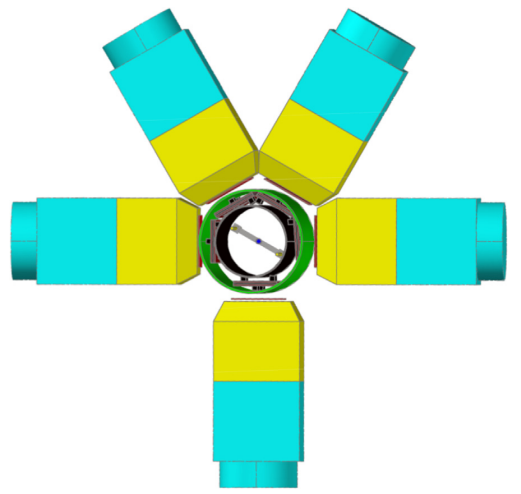
\includegraphics[width=\textwidth]{../images/atomki_detector.png}
					\end{minipage}
					\small{ATOMKI spectrometer.~\cite{atomki_det}}\\ \vspace{0.1cm}
					\tiny{Beam pipe (black), MWPC, $\Delta$E~det. (red), $E$~scintillators (yellow), light guides (blue)}
				\column{0.33 \textwidth}
					\centering
					\begin{minipage}[t][4cm]{\textwidth}
						\centering
						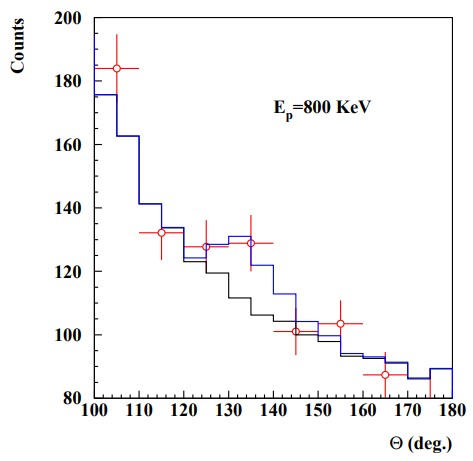
\includegraphics[width=\textwidth]{../images/atomki_be.png}
					\end{minipage}
					\footnotesize{$ {}^8\text{Be} $, $e^{+}e^{-}$ pair angular correlation.~\cite{atomki_be}}
				\column{0.28 \textwidth}
					\centering
					\begin{minipage}[t][4cm]{\textwidth}
						\centering
						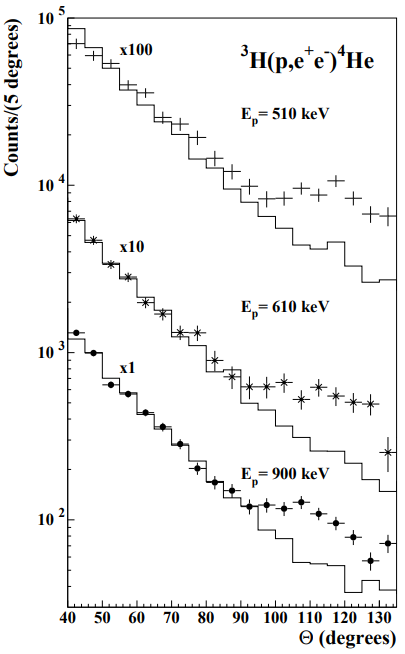
\includegraphics[width=0.7\textwidth]{../images/atomki_he.png}\newline
					\end{minipage}
					\footnotesize{$ {}^4\text{He} $, $e^{+}e^{-}$ pair angular correlation.~\cite{atomki_he}}
			\end{columns}
		\end{itemize}
	\end{frame}
	\begin{frame}
		\frametitle{OFTPC: Detector Configuration}
		\begin{itemize}
			\item Time Projection Chamber with Orthogonal Fields (OFTPC) -- electric and magnetic field perpendicular
		\end{itemize}
		\begin{columns}
			\column{0.47 \textwidth}
				\centering
				\begin{minipage}[t][4.05cm]{\textwidth}
					\centering
					\textcolor{white}{a\,\,}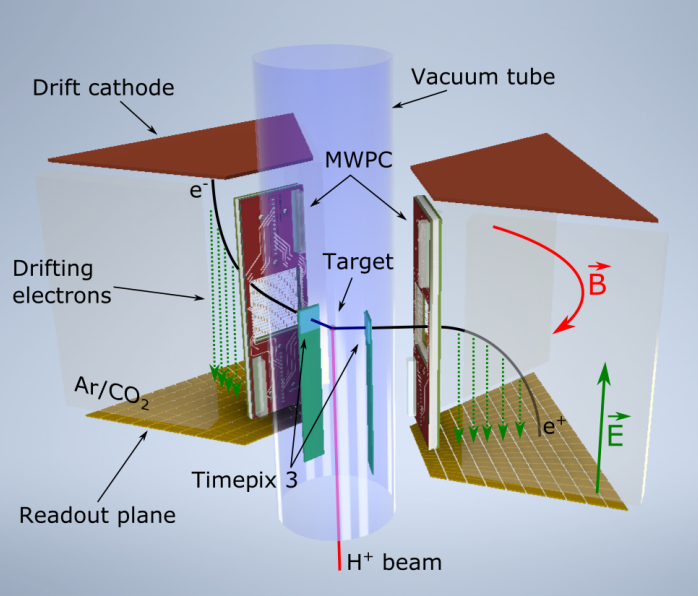
\includegraphics[width=0.82\linewidth]{../images/diagram.png}\newline
				\end{minipage}
				Two out of the six OFTPC chambers.~\cite{poster}
			\column{0.47 \textwidth}
				\centering
				\begin{minipage}[t][4.05cm]{\textwidth}
					\centering
					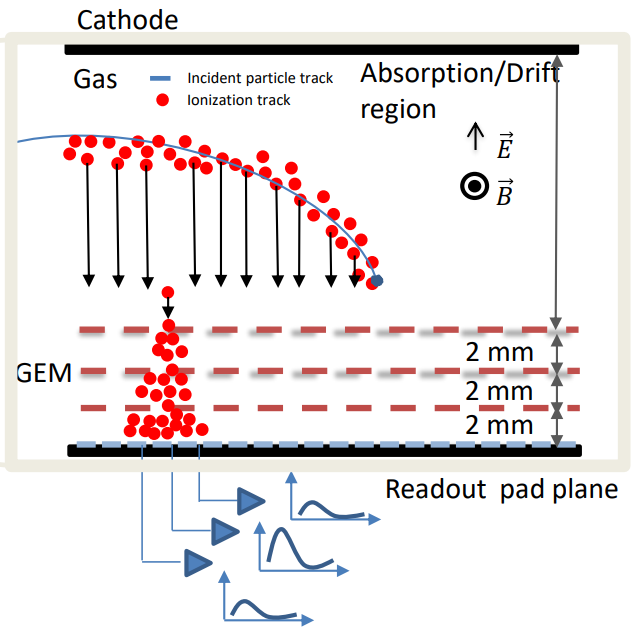
\includegraphics[width=0.71\linewidth]{../images/diagram2.png}\newline
				\end{minipage}
				OFTPC with a triple gas electron multiplier (GEM) readout.~\cite{poster}
		\end{columns}
	\end{frame}

	\begin{frame}
		\frametitle{OFTPC: Reasons for Orthogonal Fields}
		\begin{itemize}
			\item No solenoid -- permanent magnets used to generate the field
			\begin{itemize}
				\item Parallel fields difficult to create with permanent magnets
			\end{itemize}
			\item Space constraints -- granularity of the TPC readout limited in order to fit one SAMPA/SRS hybrid in each of the six sectors
			\begin{itemize}
				\item Parallel fields would bend particles parallel to readout, requiring much larger number of pads
				\item These trajectories would extend to more than one sector, requiring alternative architecture of the detector
			\end{itemize}
			\item We expect a similar resolution for significantly lower cost
		\end{itemize}
	\end{frame}
	
	\begin{frame}
		\frametitle{OFTPC: Complications}
		Inhomogeneous magnetic field (simulated using Maxwell~\textcolor{red}{Add citation!})
		\begin{columns}
			\column{0.5\textwidth}
				\centering
				\begin{minipage}[t][4cm]{\textwidth}
					\centering
					\vspace{0.4cm}
					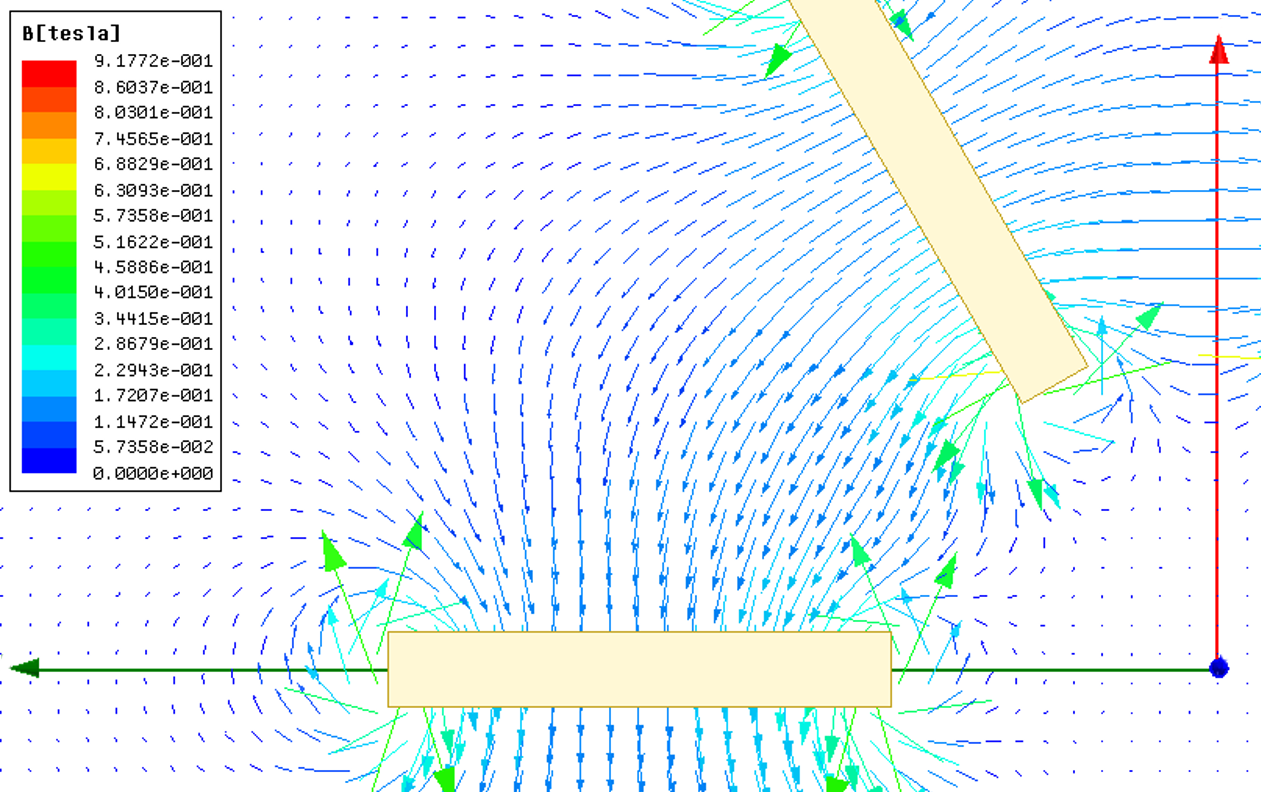
\includegraphics[width = 0.95 \textwidth]{../images/maxwell_zoom.png}
				\end{minipage}
			\column{0.5\textwidth}
				\centering
				\begin{minipage}[t][4cm]{\textwidth}
					\centering
					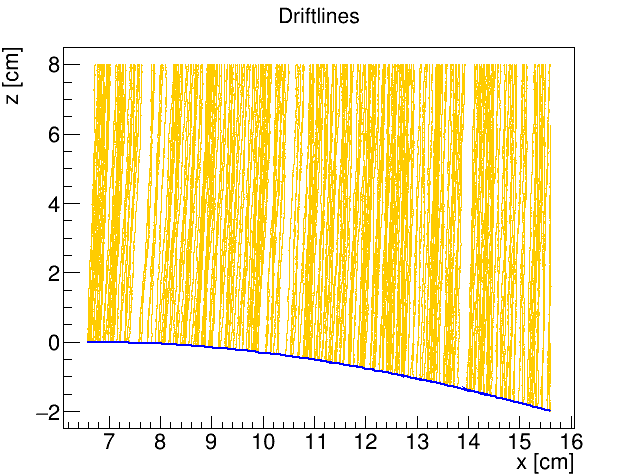
\includegraphics[width = 0.95 \textwidth]{../images/drift_xz.png}
				\end{minipage}
		\end{columns}
		\begin{itemize}
			\item The field interferes with the direction of the drift of secondary electrons
			\item Curvature of the track is not constant in this field (deviation from a~circle)
		\end{itemize}
	\end{frame}
	
	\section{Track simulation}
	\begin{frame}
		\frametitle{Track simulation}
		\begin{itemize}
			\item Garfield++ used for track simulation
			\begin{itemize}
				\item Primary relativistic particle simulated using the HEED program~\cite{heed}
				\item Secondary ionization electrons simulated using microscopic tracking (uses equations of motion)
				\begin{itemize}\item Relatively slow (typically 5-30 CPU hours per track), very precise especially for small structures.  \end{itemize}
			\end{itemize}
			\item Batches of 9702 tracks with different initial parameters simulated on a grid (MetaCentrum~\cite{meta})
			\begin{itemize}
				\item Electrons and positrons
				\item 11 different energies from 3~MeV to 13~MeV (covers range for $ {}^8\text{Be} $)
				\item 21 different angles~$\varphi$ and 21 different angles~$\theta$ (next slide)
			\end{itemize}
		\end{itemize}
	\end{frame}
	
	\begin{frame}
		\frametitle{Track simulation}
		\centering
		\large{Spherical angles ($\theta$,$\varphi$) with respect to~$z$}\\
		\small{$\theta$ taken from the equatorial plane $xy$}
		\centering
		\textcolor{white}{aaaaaaaa}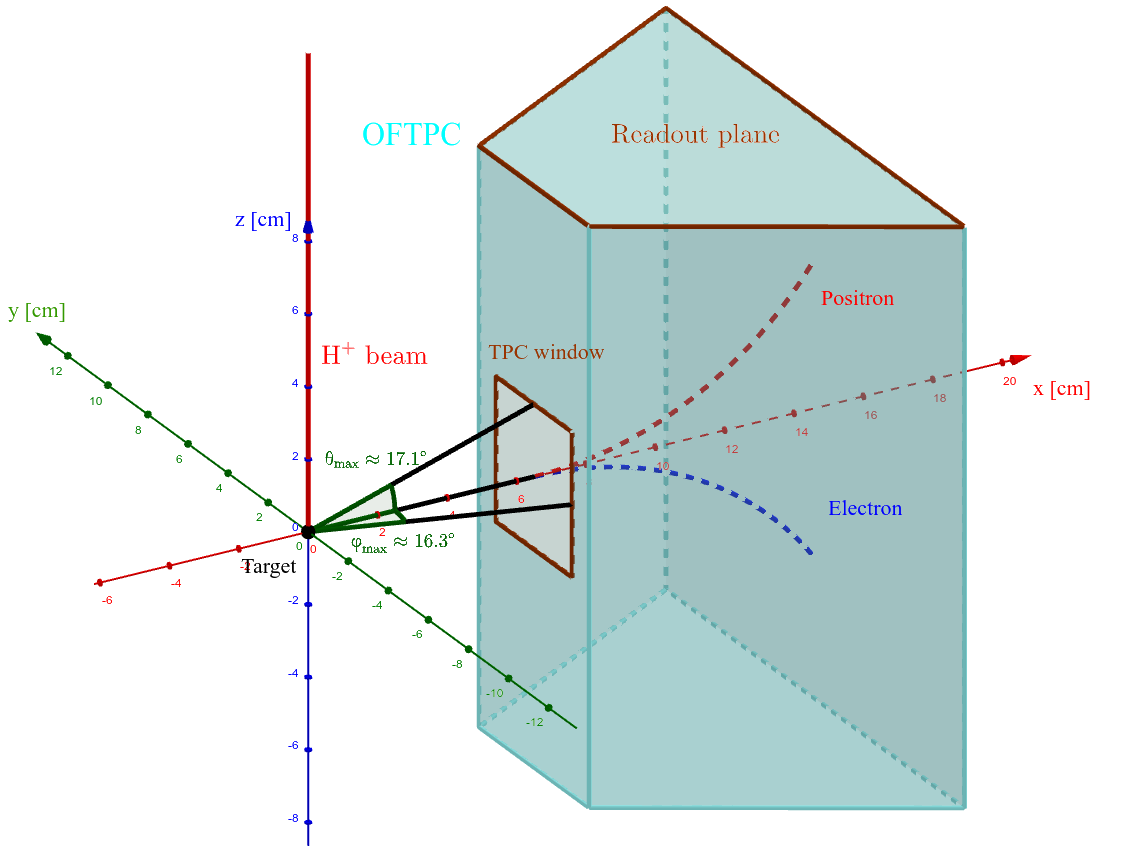
\includegraphics[height= 0.61 \textheight]{../images/tpc_micro_simulation.png}\newline
		\small{Diagram of the batch simulation parameters:\\ $\theta\in[-17.1^\circ,17.1^\circ]$, $\varphi~\in~[-16.3^\circ,16.3^\circ]$, $ E_\text{kin.} \in [3,13] $~MeV.}
	\end{frame}
	
	\begin{frame}
		\frametitle{Simulated track example (microscopic tracking)}
		\begin{itemize}
			\item Electron track with kinetic energy 8~MeV, $\theta = 0^\circ$ and $\varphi = 0^\circ$
			\item Diffusion less than 1.5~mm in both directions
		\end{itemize}
		\vspace{0.5cm}
		\begin{columns}
			\column{0.33\textwidth}
				\centering
				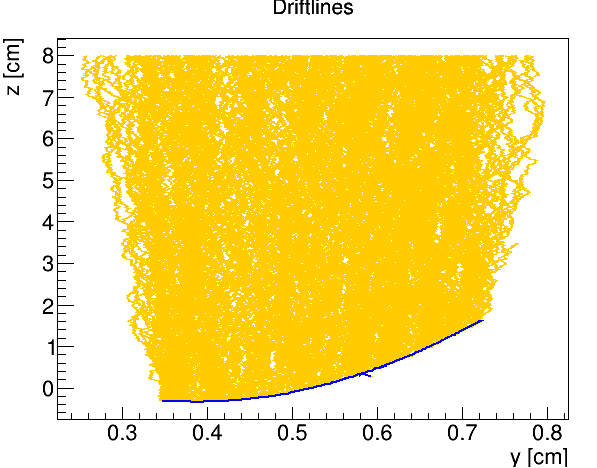
\includegraphics[width = 0.95 \linewidth]{../images/drift_yz.png}
				Diffusion front view
			\column{0.33\textwidth}
				\centering
				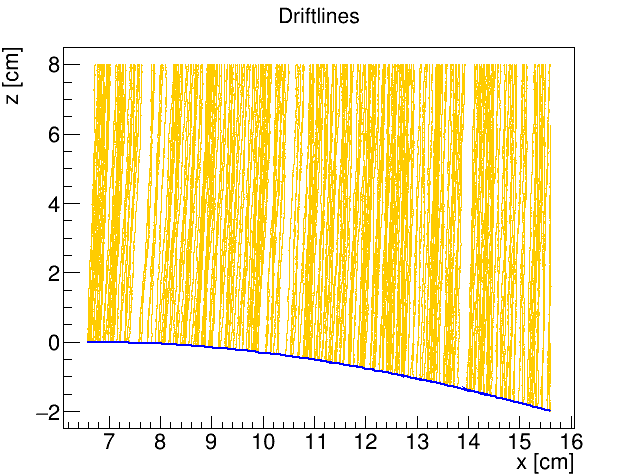
\includegraphics[width = 0.95 \linewidth]{../images/drift_xz.png}
				Electron drift
			\column{0.33\textwidth}
				\centering
				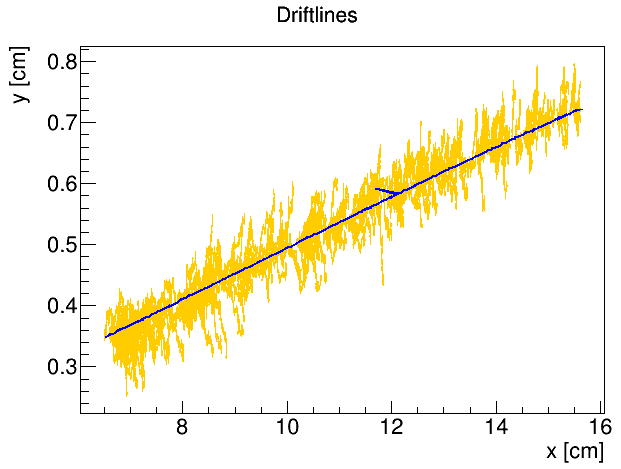
\includegraphics[width = 0.95 \linewidth]{../images/drift_xy.png}
				Diffusion top view
		\end{columns}
	\end{frame}

	\begin{frame}
		\frametitle{Ionization electrons map simulation}
		\begin{itemize}
			\item We want an~unambiguous map of the drift of secondary electrons for the reconstruction
			\item We can use a~simulation of evenly spaced electrons
			\begin{itemize}
				\item Current spacing 5~mm, 100 electrons simulated in each location with 0.1~eV energy in a~random direction
			\end{itemize}
		\end{itemize}
		\begin{columns}
			\column{0.06\textwidth}
			\column{0.44\textwidth}
				\centering
				\begin{minipage}[t][4.2cm]{\textwidth}
					\centering
					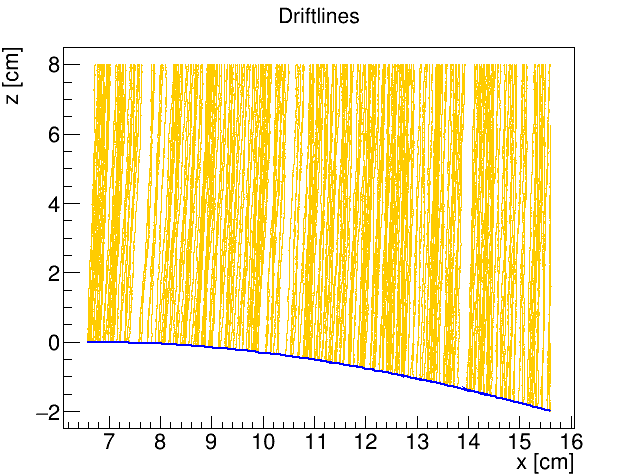
\includegraphics[width = \textwidth]{../images/drift_xz.png}\\
				\end{minipage}
				{Electron drift}
			\column{0.44\textwidth}
				\centering
				\begin{minipage}[t][4.2cm]{\textwidth}
					\centering
					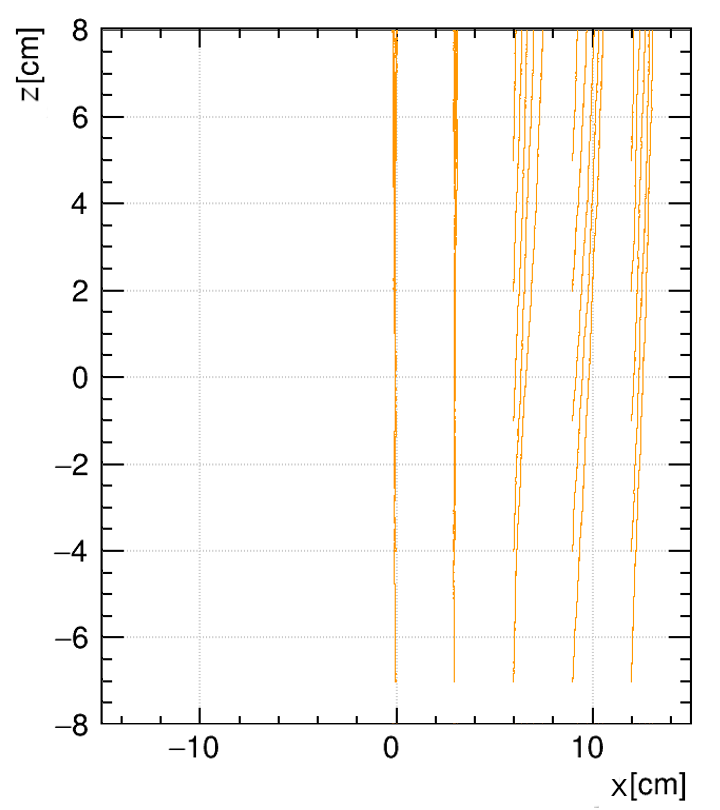
\includegraphics[width=0.7\textwidth]{../images/map_lines_flipped.png}\\
				\end{minipage}
				{Partial simulation of the map}
			\column{0.06\textwidth}
		\end{columns}
	\end{frame}

	\begin{frame}
		\frametitle{Ionization electron map simulation}
		\begin{itemize}
			\item As a result we get an approximation of a mapping from initial coordinates of the electrons $(x,y,z)$ to the readout coordinates $(x',y',t)$
			\item By interpolating we can get the inverse map
			\item We can use the inverse map to finally create mapping from our discrete readout values (channel number, time) to voxels of the primary track
		\end{itemize}
		\begin{figure}
			\centering
			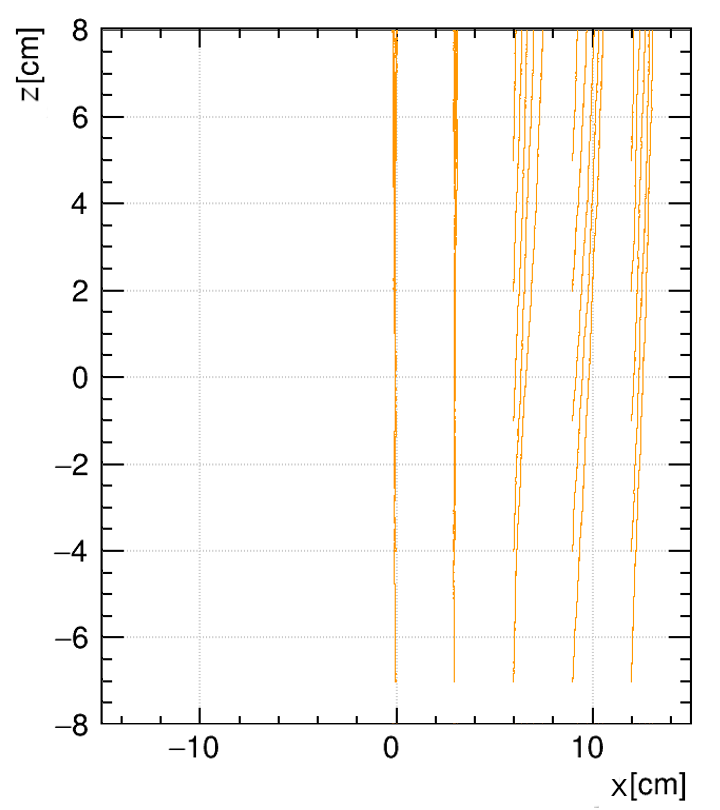
\includegraphics[height=0.4\textheight]{../images/map_lines_flipped.png}\\
			\small{Partial simulation of the map}
		\end{figure}
	\end{frame}
	\begin{frame}
		\frametitle{Ionization electron map simulation}
		\begin{figure}
			\centering
			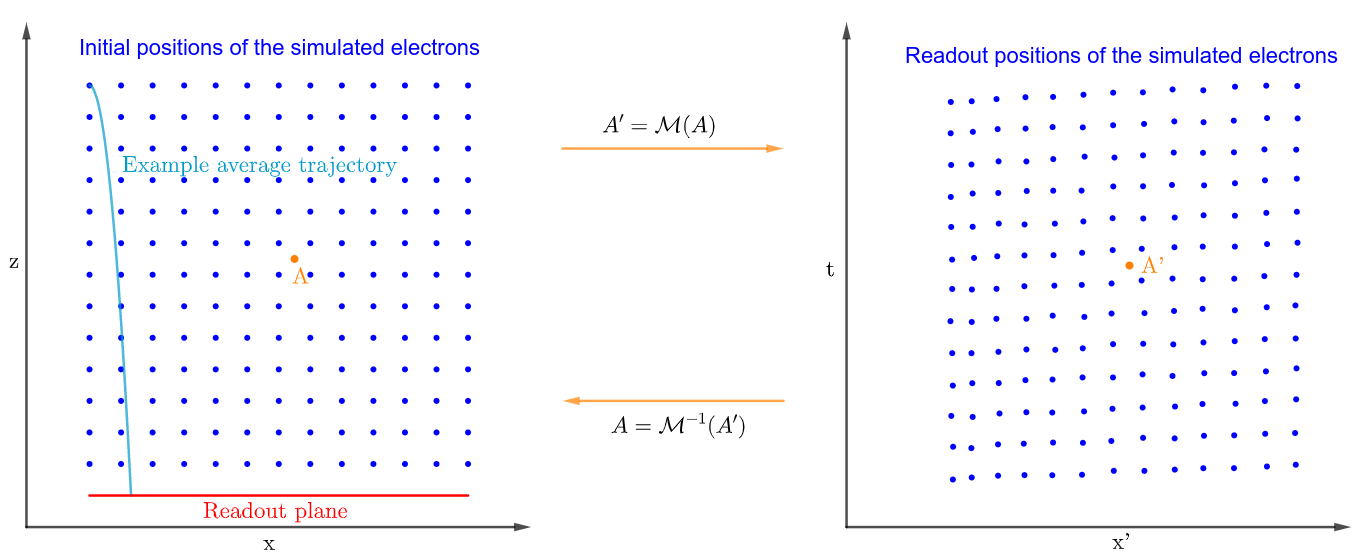
\includegraphics[width=\textwidth]{../images/map_visualization_big.png}
			\small{2D visualization of the simulated mapping $\mathcal{M}$ and the inverse mapping $\mathcal{M}^{-1}$.}
		\end{figure}
	\end{frame}
	\begin{frame}
		\frametitle{Ionization electron map simulation}
		\begin{figure}
			\centering
			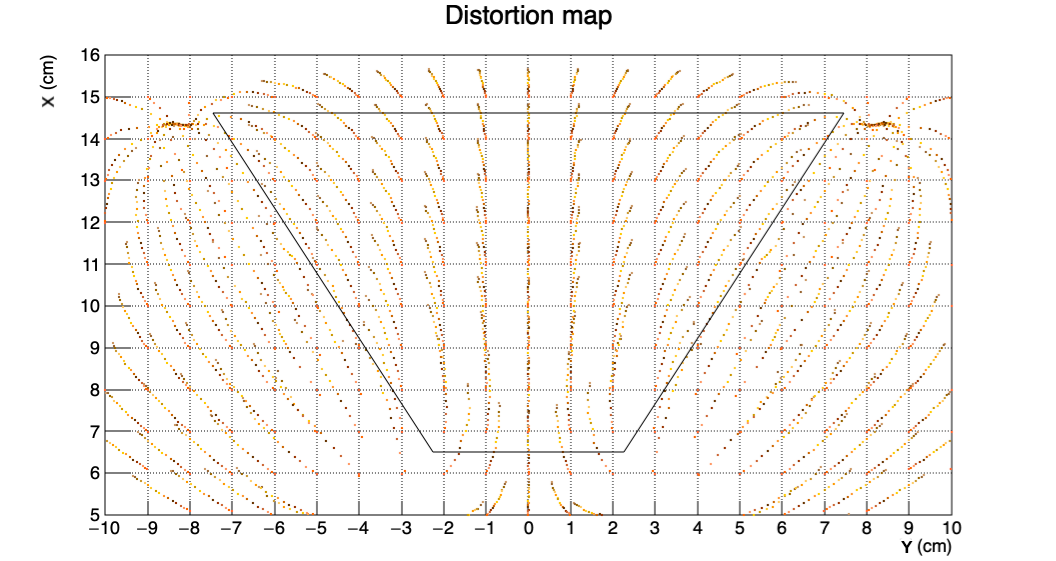
\includegraphics[height=0.68\textheight]{../images/map_dist.png}\\
			\small{$x$ and $y$ coordinate distortion at different $z$ values (denoted by colors).}
		\end{figure}
	\end{frame}
	\begin{frame}
		\frametitle{Ionization electron map simulation}
		\centering
		\begin{minipage}[c]{0.9\textwidth}
			\begin{figure}
				\centering
				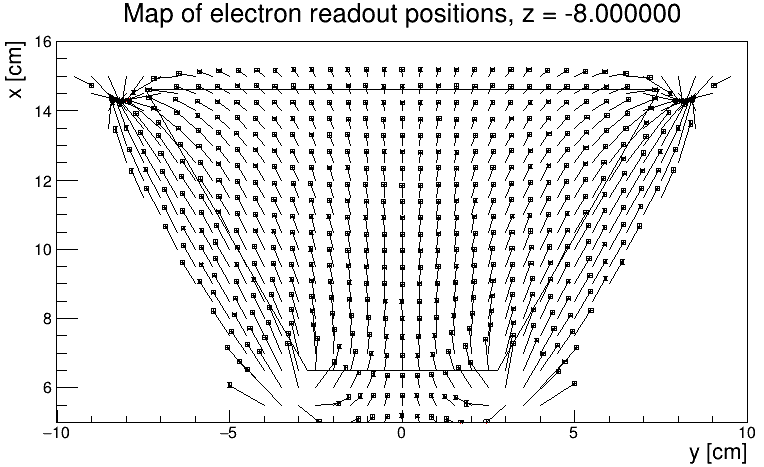
\includegraphics[height=0.7\textheight]{../images/map_dist2_new.png}\\
				\small{Worst case $x$ and $y$ coordinate distortion for maximal initial distance from readout.}
			\end{figure}
		\end{minipage}
	\end{frame}
	\begin{frame}
		\frametitle{Ionization electron map simulation}
		\begin{figure}
			\centering
			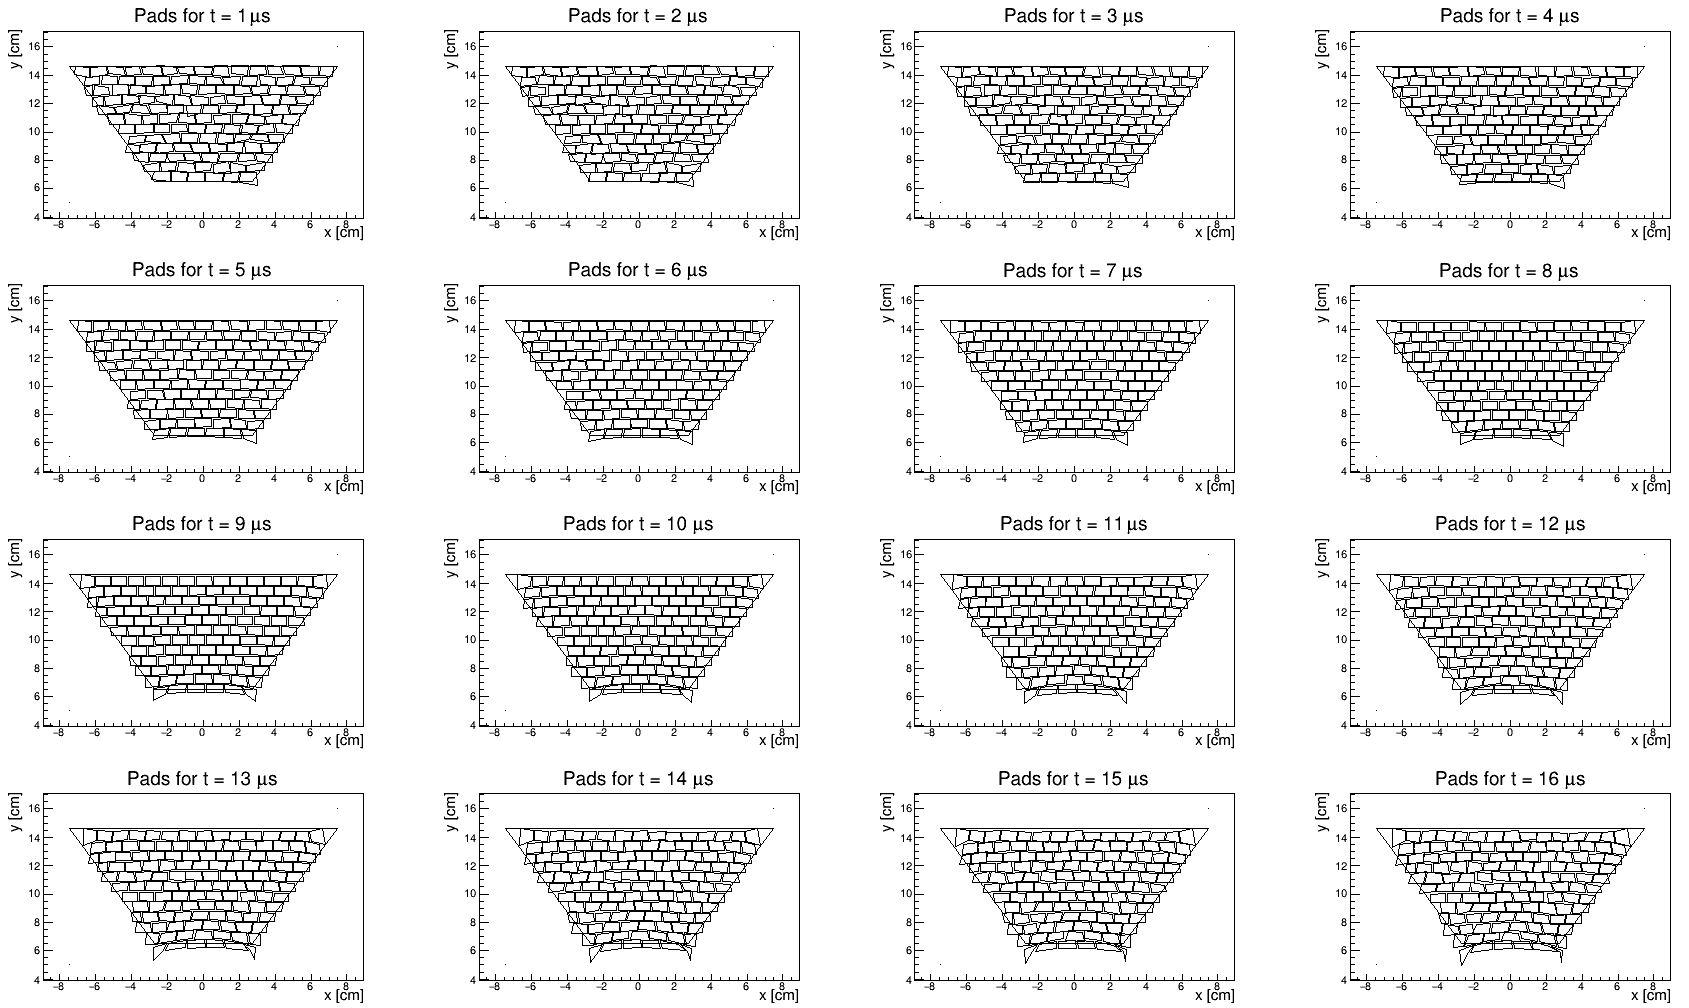
\includegraphics[height=0.68\textheight]{../images/pads_distortion.png}\\
			{Pad voxel boundaries for different times.}
		\end{figure}
	\end{frame}


	\section{Track reconstruction}
	\begin{frame}
		\frametitle{Track reconstruction}
		\begin{itemize}
			\item At first using only the inverse map (not accounting for readout pads)
			\item Later simple reconstruction with pads and time bins, counting the number of electrons in each bin
		\end{itemize}
		\begin{columns}
			\column{0.5\textwidth}
				\centering
				\begin{minipage}[t][4.5cm]{\textwidth}
					\centering
					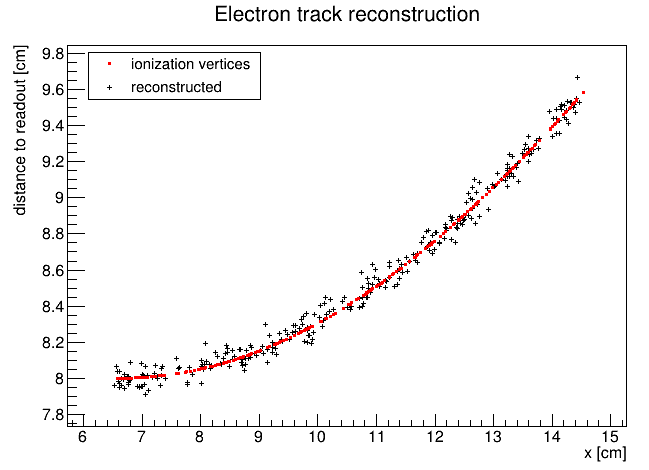
\includegraphics[width=\textwidth]{../images/reco_track_new.png}\\
				\end{minipage}
				\small{Original and reconstructed interaction points on the simulated track}
			\column{0.5\textwidth}
				\centering
				\begin{minipage}[t][4.5cm]{\textwidth}
					\centering
					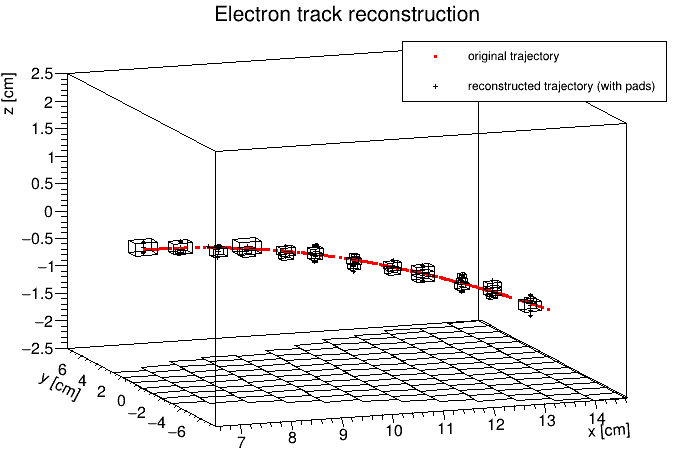
\includegraphics[width=\textwidth]{../images/reco_track_pads.png}\\
				\end{minipage}
				\small{Reconstruction with pads}
		\end{columns}
	\end{frame}

	\section{Energy reconstruction}
	\begin{frame}
		\frametitle{Energy reconstruction}
		\begin{itemize}
			\item Prefit with circle with smoothly attached lines
			\item Kinetic energy fit using 4\textsuperscript{th} order Runge-Kutta
			\item Known initial position and direction of the particle assumed
			\item Currently cca 0.3~CPU seconds per track
		\end{itemize}
		\begin{columns}
			\column{0.5\textwidth}
				\centering
				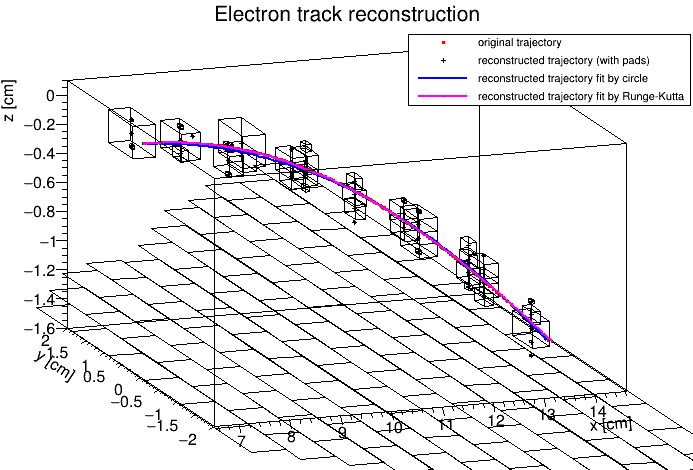
\includegraphics[width=\textwidth]{../images/reco_track_pads2.png}\\
			\column{0.5\textwidth}
				\centering
				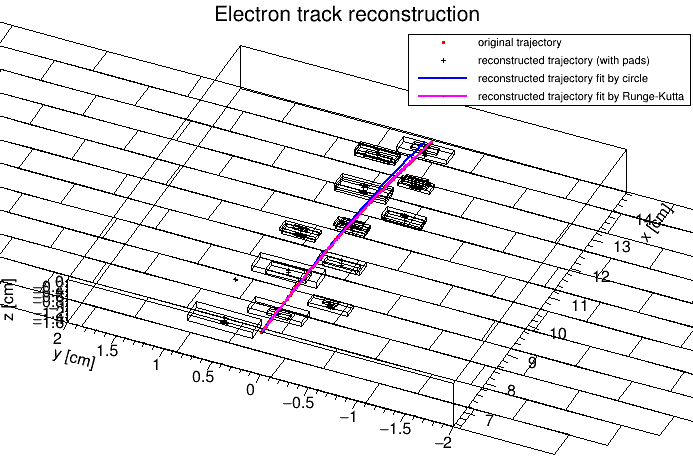
\includegraphics[width=\textwidth]{../images/reco_track_pads3.png}\\
		\end{columns}
		\vspace{0.5cm}
		\centering
		\begin{minipage}{0.8\textwidth}
			\centering
			\small{Energy reconstruction of 8~MeV electron track with both circle fit (8.36~MeV) and Runge-Kutta fit (8.072~MeV)}
		\end{minipage}
	\end{frame}
	\begin{frame}
		\frametitle{Energy reconstruction precision}
		\centering
		\begin{columns}
			\column{0.5\textwidth}
			\centering
			\Large \textbf{Electrons}
			\begin{figure}
				\centering
				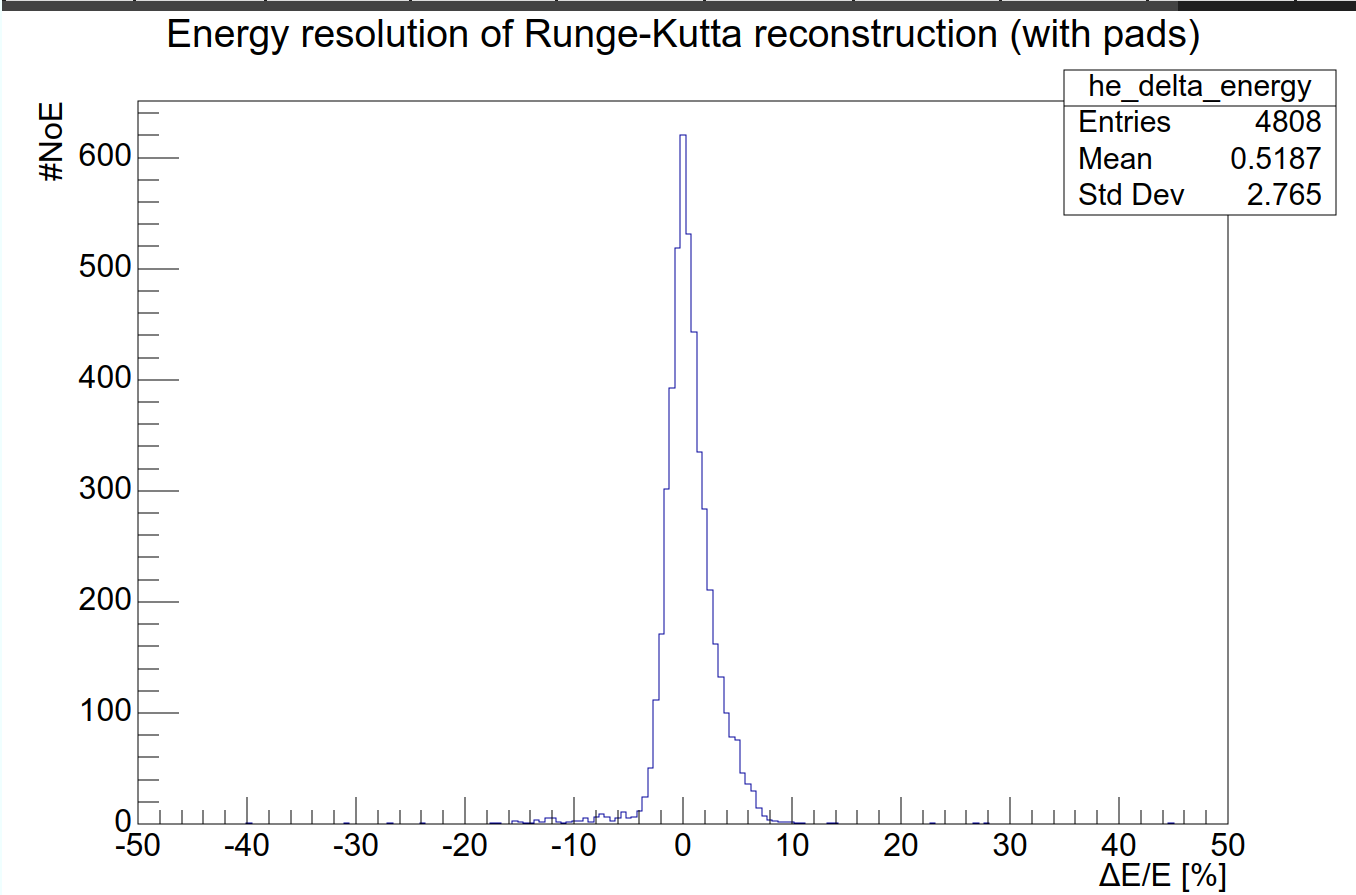
\includegraphics[width = 0.95 \linewidth]{../images/c_e_delta_energy.png}
			\end{figure}
			\column{0.5\textwidth}
			\centering
			\Large \textbf{Positrons}
			\begin{figure}
				\centering
				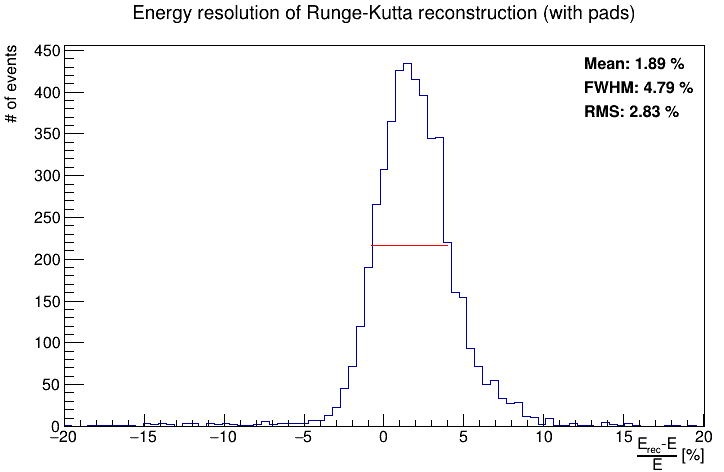
\includegraphics[width = 0.95 \linewidth]{../images/c_p_delta_energy.png}
			\end{figure}
		\end{columns}
		\vspace{0.5cm}
		\footnotesize{Relative reconstruction deviation of the~kinetic energy of electron and positron tracks (cca 5000 of each simulated).}
	\end{frame}
	\begin{frame}
		\frametitle{Energy reconstruction precision}
		\centering
		\begin{columns}
			\column{0.5\textwidth}
			\centering
			\Large \textbf{Electrons}
			\begin{figure}
				\centering
				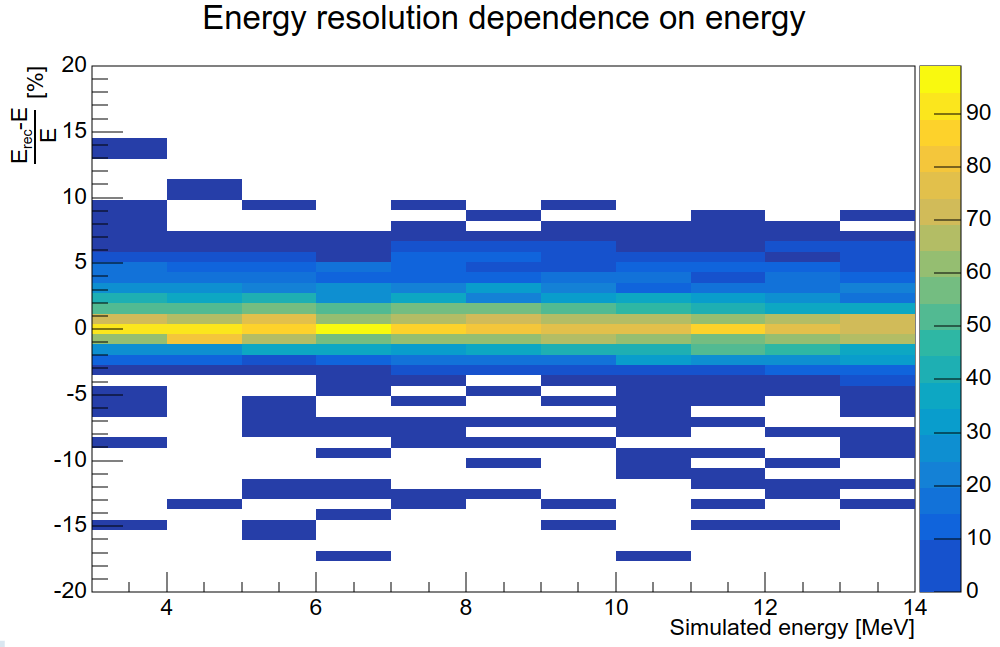
\includegraphics[width = 0.95 \linewidth]{../images/h_e_deltaenergy_energy.png}
			\end{figure}
			\column{0.5\textwidth}
			\centering
			\Large \textbf{Positrons}
			\begin{figure}
				\centering
				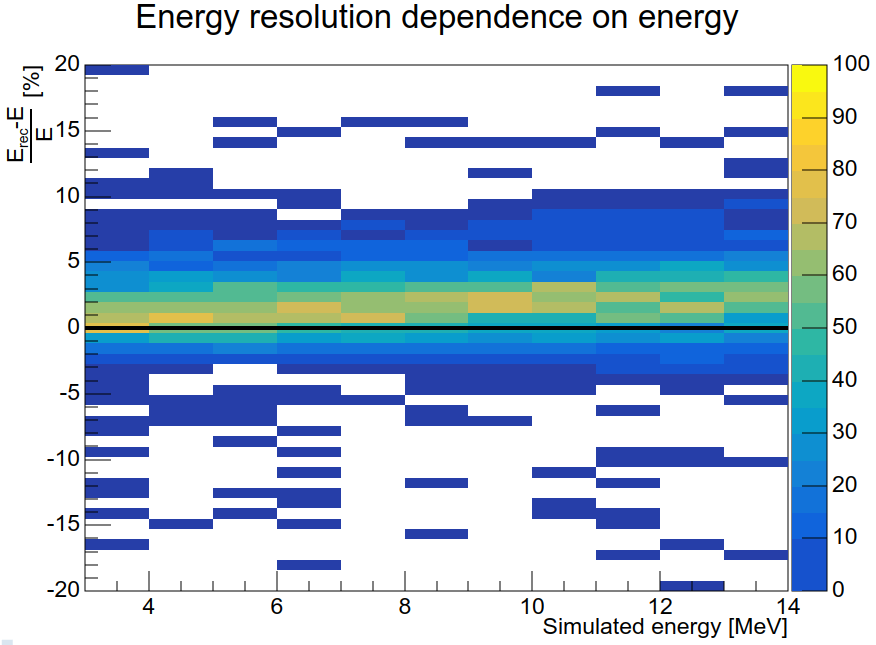
\includegraphics[width = 0.95 \linewidth]{../images/h_p_deltaenergy_energy.png}
			\end{figure}
		\end{columns}
		\vspace{0.5cm}
		\footnotesize{Relative reconstruction deviation of the~kinetic energy of electron and positron tracks (cca 5000 of each simulated).}
	\end{frame}
	\begin{frame}
		\frametitle{Energy reconstruction precision}
		\centering
		\begin{columns}
			\column{0.5\textwidth}
			\centering
			\Large \textbf{Electrons}
			\begin{figure}
				\centering
				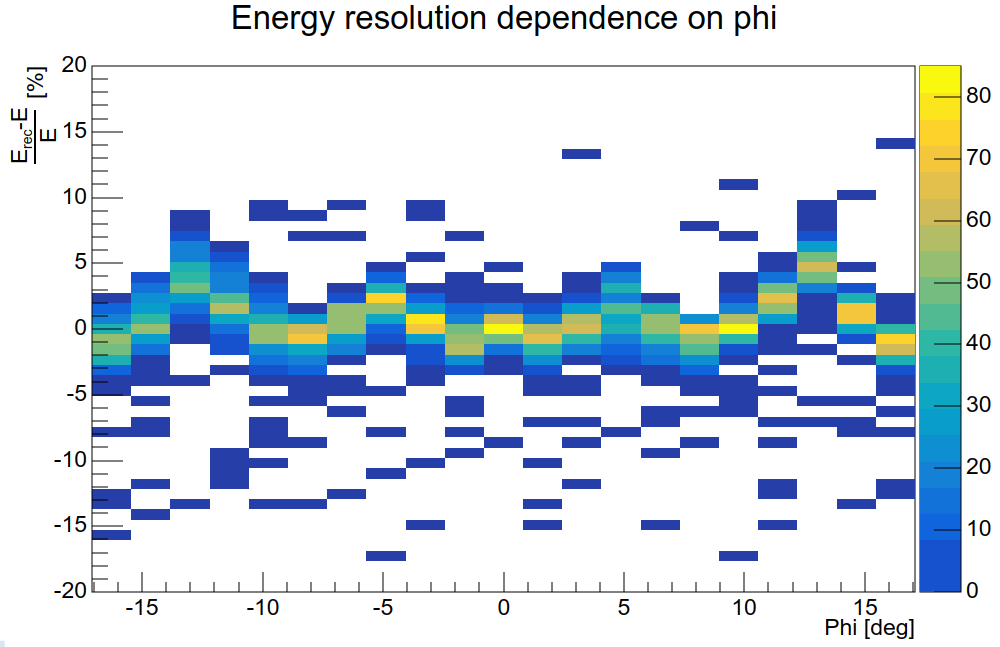
\includegraphics[width = 0.95 \linewidth]{../images/h_e_deltaenergy_phi.png}
			\end{figure}
			\column{0.5\textwidth}
			\centering
			\Large \textbf{Positrons}
			\begin{figure}
				\centering
				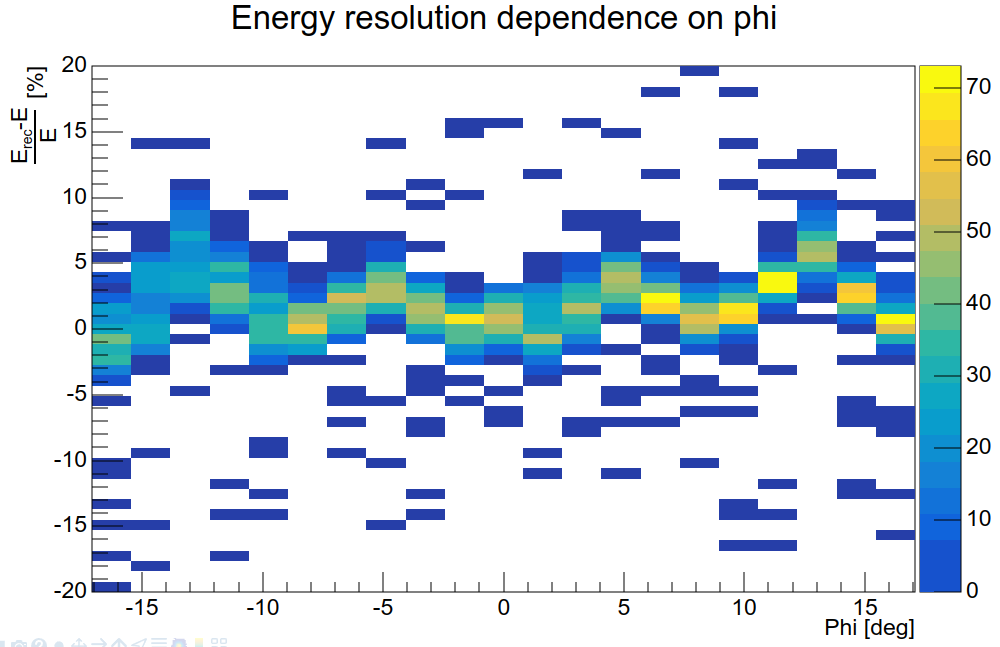
\includegraphics[width = 0.95 \linewidth]{../images/h_p_deltaenergy_phi.png}
			\end{figure}
		\end{columns}
		\vspace{0.5cm}
		\footnotesize{Relative reconstruction deviation of the~kinetic energy of electron and positron tracks (cca 5000 of each simulated).}
	\end{frame}
	\begin{frame}
		\frametitle{Energy reconstruction precision}
		\centering
		\begin{columns}
			\column{0.5\textwidth}
			\centering
			\Large \textbf{Electrons}
			\begin{figure}
				\centering
				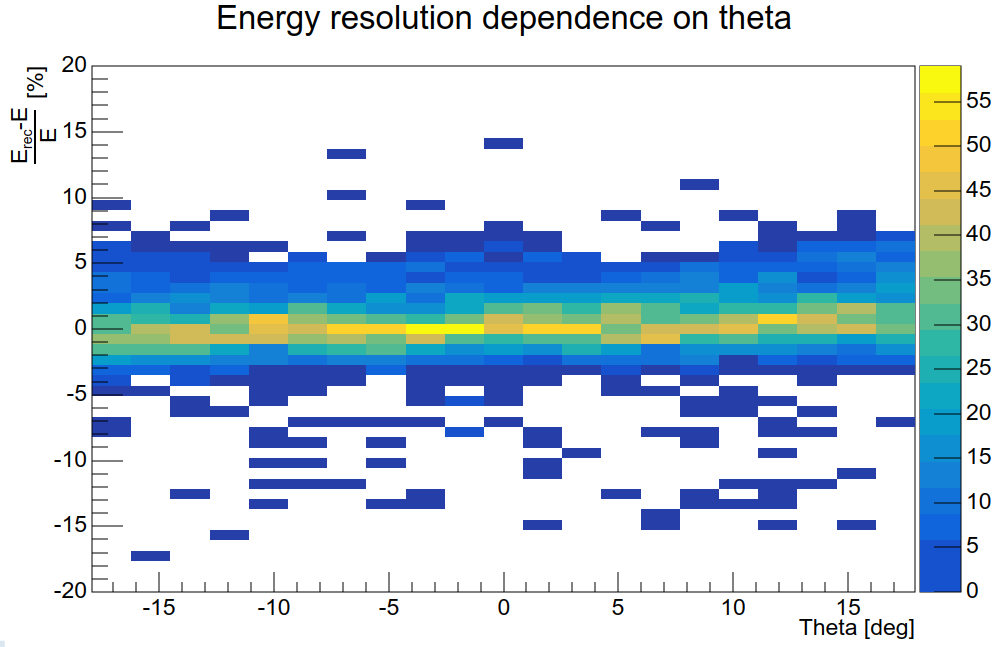
\includegraphics[width = 0.95 \linewidth]{../images/h_e_deltaenergy_theta.png}
			\end{figure}
			\column{0.5\textwidth}
			\centering
			\Large \textbf{Positrons}
			\begin{figure}
				\centering
				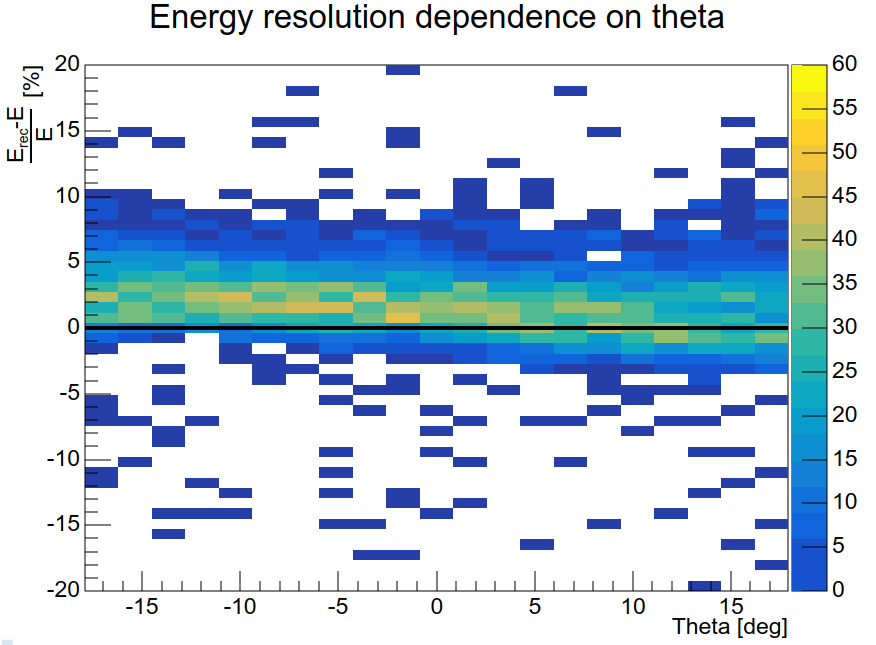
\includegraphics[width = 0.95 \linewidth]{../images/h_p_deltaenergy_theta.png}
			\end{figure}
		\end{columns}
		\vspace{0.5cm}
		\footnotesize{Relative reconstruction deviation of the~kinetic energy of electron and positron tracks (cca 5000 of each simulated).}
	\end{frame}
	
	
	\section{Summary \& Future}	
	\begin{frame}
		\frametitle{Summary}
		\begin{itemize}
			\item Several batches of tracks have been simulated for testing purposes.
			\begin{itemize}
				\item $\theta\in[-17.1^\circ,17.1^\circ]$, $\varphi~\in~[-16.3^\circ,16.3^\circ]$, $ E_k \in [3,13] $~MeV
			\end{itemize}
			\item The map of secondary electron positions and drift times has been generated.
			\item The map has been tested by the track reconstruction.
			\item First results suggest that:
			\begin{itemize}
				\item Current energy resolution (FWHM) is 3.2~\% for electrons and 4.8~\% for positrons.
				\item OFTPC works well on a simulation level.
			\end{itemize}
		\end{itemize}
	\end{frame}
	\begin{frame}
		\frametitle{Future Steps}
		\begin{itemize}
			\item Account for parasitic tracks caused by high energy secondary electrons
			\item Account for GEM in the simulation, charge distribution between pads
			\item Optimize Runge-Kutta integration fit with likelihood approach (instead of least squares) if needed
			\item Write a faster simulation method for secondary electrons using the map
			\item Fix the observed systematic error of reconstruction
		\end{itemize}
	\end{frame}
	
	{
		%\usebackgroundtemplate{\includegraphics[width=\paperwidth,height=\paperheight]{../images/DSC_5602.jpg}}%
		\begin{frame}[noframenumbering]{}
			\begin{center}
				\Huge Thank you for your attention.
			\end{center}
		\end{frame}
	}
	
	%\section{References}
	\begin{frame}[allowframebreaks,noframenumbering]
		\frametitle{References}
		%\printbibliography
		\bibliography{../references}
		\bibliographystyle{unsrt}
	\end{frame}
	\begin{frame}[noframenumbering]
	\frametitle{Notes (what else to mention)}
		\begin{itemize}
			\item Extra slide with the whole process summary?
			\item Better description than pad voxels.
			\item Residues on first attempts of track reconstruction?
		\end{itemize}
	\end{frame}
	
\end{document}